\newpage
МРНТИ 06.73.93
\hfill {\bfseries \href{https://doi.org/10.58805/kazutb.v.3.24-569}{https://doi.org/10.58805/kazutb.v.3.24-569}}

\sectionwithauthors{А. М. Курманов, И. Е.Сарыбаева, А. Н. Омаркожаева, А.Б. Бекмагамбетов}{СОВЕРШЕНСТВОВАНИЕ СИСТЕМЫ УЧЕТА И АНАЛИЗА ЗАТРАТ НА ОХРАНУ ТРУДА В РЕСПУБЛИКЕ КАЗАХСТАН: ПРОБЛЕМЫ, ПЕРСПЕКТИВЫ И СТРАТЕГИИ УЛУЧШЕНИЯ}

\begin{center}
{\bfseries \textsuperscript{1}А. М. Курманов, \textsuperscript{2}И.
Е.Сарыбаева\envelope, \textsuperscript{3}А. Н. Омаркожаева,
\textsuperscript{1}А.Б. Бекмагамбетов}

\textsuperscript{1} Республиканский научно-исследовательский институт по
охране труда Министерства труда и социальной защиты населения Республики
Казахстан, Астана, Казахстан,

\textsuperscript{2} Евразийский национальный университет имени Л.Н.
Гумилева, Астана, Казахстан,

\textsuperscript{3} Казахский университет технологии и бизнеса
им.К.Кулажанова, Астана, Казахстан
\end{center}

\envelope Корреспондент-автор:
inarasaribaeva@gmail.com

В статье рассматриваются проблемы и перспективы совершенствования
системы социальных гарантий для работников, занятых на вредных и опасных
производствах в Республике Казахстан. На основе анализа текущего
законодательства и практики предоставления компенсаций выявлены
существенные недостатки, связанные с отсутствием единого подхода к
аттестации рабочих мест и недостаточной объективностью оценки условий
труда. Особое внимание уделяется необходимости разработки
унифицированных стандартов и критериев оценки, усилению контроля за
проведением аттестации, а также внедрению дифференцированного подхода к
предоставлению социальных гарантий. В статье предложены рекомендации по
совершенствованию системы, которые включают разработку новых
законодательных актов, повышение квалификации специалистов по охране
труда и создание механизмов обратной связи для работников. Эти меры
направлены на обеспечение более справедливых и равных условий труда, что
в конечном итоге способствует улучшению производственной среды и
снижению уровня профессиональных заболеваний.

{\bfseries Ключевые слова:} социальные гарантии, вредные и опасные условия
труда, компенсации, охрана труда, аттестация рабочих мест, условия труда

\sectionheading{ҚАЗАҚСТАН РЕСПУБЛИКАСЫНДА ЕҢБЕКТІ ҚОРҒАУҒА АРНАЛҒАН ШЫҒЫНДАРДЫ
ЕСЕПКЕ АЛУ ЖӘНЕ ТАЛДАУ ЖҮЙЕСІН ЖЕТІЛДІРУ: ПРОБЛЕМАЛАР, ПЕРСПЕКТИВАЛАР
ЖӘНЕ ЖАҚСАРТУ СТРАТЕГИЯЛАРЫ}

\begin{center}
{\bfseries \textsuperscript{1}А. М. Курманов, \textsuperscript{2}И. Е.
Сарыбаева\envelope, \textsuperscript{3}А. Н. Омарқожаева,
\textsuperscript{1}А.Б. Бекмағамбетов}

\textsuperscript{1} Қазақстан Республикасы Еңбек және халықты әлеуметтік
қорғау министрлігінің Еңбекті қорғау жөніндегі республикалық
ғылыми-зерттеу институты, Астана, Қазақстан,

\textsuperscript{2} Л. Н. Гумилев атындағы Еуразия Ұлттық Университеті,
Астана, Қазақстан,

\textsuperscript{3} Қазақ технология және бизнес университеті.Қ.
Құлажанова, Астана, Қазақстан,

e-mail: inarasaribaeva@gmail.com
\end{center}

Мақалада Қазақстан Республикасындағы зиянды және қауіпті өндірістерде
жұмыс істейтін қызметкерлер үшін әлеуметтік кепілдіктер жүйесін
жетілдіру мәселелері мен перспективалары қарастырылады. Ағымдағы
заңнаманы және өтемақы беру практикасын талдау негізінде жұмыс орындарын
аттестаттауға бірыңғай тәсілдің болмауына және еңбек жағдайларын
бағалаудың объективтілігінің жеткіліксіздігіне байланысты елеулі
кемшіліктер анықталды. Бірыңғай стандарттар мен бағалау критерийлерін
әзірлеу, аттестаттауды өткізуді бақылауды күшейту, сондай-ақ әлеуметтік
кепілдіктер беруге сараланған тәсілді енгізу қажеттілігіне ерекше назар
аударылады. Мақалада жаңа заңнамалық актілерді әзірлеуді, еңбекті қорғау
жөніндегі мамандардың біліктілігін арттыруды және қызметкерлер үшін кері
байланыс тетіктерін құруды қамтитын жүйені жетілдіру бойынша ұсыныстар
ұсынылған. Бұл шаралар неғұрлым әділ және тең еңбек жағдайларын
қамтамасыз етуге бағытталған, бұл сайып келгенде өндірістік ортаны
жақсартуға және кәсіптік аурулардың деңгейін төмендетуге ықпал етеді.

{\bfseries Негізгі сөздер:} әлеуметтік кепілдіктер, зиянды және қауіпті
еңбек жағдайлары, өтемақылар, еңбекті қорғау, жұмыс орындарын
аттестаттау, еңбек жағдайлары

\sectionheading{IMPROVING THE SYSTEM OF ACCOUNTING AND ANALYSIS OF LABOR
PROTECTION COSTS IN THE REPUBLIC OF KAZAKHSTAN: PROBLEMS, PROSPECTS AND
IMPROVEMENT STRATEGIES}

\begin{center}
{\bfseries \textsuperscript{1}A.M.Kurmanov, \textsuperscript{2}I.E.
Sarybayeva\envelope, \textsuperscript{3}A.N. Omarkozhayeva,
\textsuperscript{1}A.B.Bekmagambetov}

\textsuperscript{1} Republican Research Institute for labor protection
of the Ministry of Labor and social protection of the population of the
Republic of Kazakhstan, Astana, Kazakhstan,

\textsuperscript{2} L. N. Gumilyov Eurasian National University, Astana,
Kazakhstan,

\textsuperscript{3} K.Kulazhanov Kazakh University of Technology and
Business, Astana, Kazakhstan,

e-mail: inarasaribaeva@gmail.com
\end{center}

The article discusses the problems and prospects of improving the system
of social guarantees for workers employed in hazardous and hazardous
industries in the Republic of Kazakhstan. Based on the analysis of
current legislation and the practice of providing compensation,
significant shortcomings have been identified related to the lack of a
unified approach to workplace certification and insufficient objectivity
in assessing working conditions. Special attention is paid to the need
to develop unified standards and evaluation criteria, strengthen control
over certification, as well as introduce a differentiated approach to
the provision of social guarantees. The article offers recommendations
for improving the system, which include the development of new
legislative acts, professional development of occupational safety
specialists and the creation of feedback mechanisms for employees. These
measures are aimed at ensuring fairer and more equal working conditions,
which ultimately contributes to improving the working environment and
reducing occupational diseases.

{\bfseries Key words:} social guarantees, harmful and dangerous working
conditions, compensation, labor protection, certification of workplaces,
working conditions

\begin{multicols}{2}
{\bfseries Введение.} Вопросы исследования социальных гарантий для
работников, занятых на вредных производствах труда, являются крайне
важными и многоаспектными, что обусловлено в первую очередь обеспечением
благосостояния и защиты здоровья работников. На фоне развития
промышленности и внедрения новых производственных технологий, характер и
степень воздействия на здоровье работников также изменяются, что требует
пересмотра и обновления социальных гарантий. Кроме того, важным аспектом
является обеспечение справедливости и равенства в распределении таких
гарантий среди всех категорий работников, занятых на вредных
производствах. Это связано с необходимостью учета индивидуальных
факторов риска и особенностей различных отраслей.

В соответствии со статьей 181 Трудового кодекса РК {[}1{]} работник
имеет право на рабочее место, оборудованное в соответствии с
требованиями по безопасности и охране труда, обеспечение
санитарно-бытовыми помещениями, средствами индивидуальной и коллективной
защиты в соответствии с требованиями законодательства, а также трудовым,
коллективным договорами. А по статье 182 работодателю вменяется в
обязанность проведение постоянного мониторинга уровня профессиональных
рисков с целью его профилактики, а также замены применяемых опасных
технологий и производственного оборудования на более безопасные.

Несмотря на принятые новые законодательные акты {[}2,3{]} социальные
гарантии в Казахстане по-прежнему не соответствуют ожиданиям и
потребностям работников и не обеспечивают выполнение международных норм,
не учитывают современное состояние производства и производственной
среды, условия труда на рабочих местах.

Социальные гарантии играют важную роль в уменьшении неравенства,
вызванного различиями в условиях труда, и поддерживают социальное
равновесие. В условиях модернизации производственных процессов и
изменений в трудовом законодательстве возникает необходимость пересмотра
и адаптации социальных гарантий, чтобы они оставались эффективными и
актуальными в новых социально-экономических реалиях.

Таким образом, исследование социальных гарантий для работников, занятых
на вредных производствах труда, имеет ключевое значение для развития
социальной политики и охраны труда, а его результаты могут стать основой
для принятия более эффективных и справедливых решений в данной области.

{\bfseries Материалы и методы.} Темой исследования занимались и занимаются
до сих пор как отдельные ученые, так проектные организации,
научно-исследовательские институты. Большое число публикаций посвящены
вопросам охраны труда, но теме «совершенствование регулированию труда
работников вредного и опасного производства» посвящены единичные труды.
Более того, вся изученная литература является справочной, либо
теоретические работы посвящены, как правило, решению каких-либо
отдельных вопросов, так или иначе касающихся вопросов охраны и условий
труда.

Анализ действующего механизма регулирования труда лиц, занятых в
неблагоприятных условиях изучены как отечественными, так и зарубежными
специалистами. Среди российских работ можно отметить статьи А.М. Елина,
С.С. Сергеевой «Специальная оценка условий труда: практика и итоги»
{[}4{]}, Л.И. Хайруллина, В.С. Гасилова, Тучковой О.А. «Компенсации за
работу во вредных условиях труда: основные аспекты вопроса» {[}5{]},
С.М.Ильина, Н.А., Самарской и др. «Направления совершенствования системы
предоставления гарантий и компенсаций работникам за работу в опасных
(вредных) условиях труда» {[}6{]}. Подобные исследования проводятся
также учеными странами СНГ в частности, статья Стратулата В. И.
«Социальные компенсации за вредные условия труда в Молдове» {[}7{]},
Алиевой Л. М. «Компенсационные механизмы для работников во вредных
условиях труда в Азербайджане» {[}8{]}, Умарова Н. А. «Правовые аспекты
компенсации за вредные условия труда в Узбекистане» {[}9{]} и др. В
Казахстане можно отметить, следующие исследования С.Г. Бисакаева, Ш.К.
Абикеновой, Каминскаой Г. А. «Научное обоснование механизма
государственного регулирования труда работников, занятых во вредных
условиях труда» {[}10{]}, Г.А. Еселхановой, А.Е. Танабаевой
«Нормативно-правовое регулирование предоставления гарантий работникам,
занятым во вредных и опасных условиях труда в Республике Казахстан»
{[}11{]}, С.М. Базарбаевой, С.Т. Шорманова, С.Т. Толеугали «Анализ
действующего механизма регулирования труда лиц, занятых в
неблагоприятных условиях» {[}12{]}.

Можно отметить ряд работ ученых дальнего зарубежья Lee, H. S., Kim, J.
H. «Occupational hazards and safety management in the South Korean
manufacturing sector» (Южная Корея) {[}13{]}, Leigh, J. P., Du, J.
«Economic burden of occupational injuries and illnesses in the United
States» {[}14{]} (США), Pissarides, C. A., Weber, A. «Compensation for
workplace risks in the European Union: Evidence from the European
Working Conditions Survey» {[}15{]} (Европа) и др.

Таким образом, в данном исследовании использовались различные источники
и методы для анализа действующего механизма регулирования труда лиц,
занятых в неблагоприятных условиях. Характеристика исследовательского
материала включает в себя как качественные, так и количественные
аспекты, что является важным фактором для обеспечения достоверности
выводов и методов исследования.

Исследование проводилось в несколько этапов: анализ существующих
законодательных актов, сбор и анализ статистических данных по
численности работников, занятых во вредных условиях труда, и
сравнительный анализ компенсационных механизмов.

При написании статьи использовались следующие методы: документальный
анализ правовых актов, статистический анализ данных по численности
работников, занятых во вредных условиях труда, и их компенсации,
сравнительный анализ компенсаций по различным формам собственности
предприятий.

{\bfseries Результаты и обсуждение.} Социальная защита работников, занятых
на тяжелых работах, а также на работах с вредными и (или) опасными
условиями труда, является одной из важнейших задач государственной
политики в сфере трудовых отношений в Республике Казахстан.
Нормативно-правовое регулирование в этой области направлено на создание
условий, обеспечивающих здоровье и безопасность работников, а также на
предоставление им дополнительных социальных гарантий и компенсаций.

Нормативно-правовой анализ исследования регуляторных норм, действующих в
Республике Казахстан представлен в таблице 1.
\end{multicols}

\begin{longtable}[c]{|lp{0.5\textwidth}|}
\caption*{Таблица 1 - Нормативно-правовой анализ регуляторных норм в сфере охраны труда} \\
\hline
\multicolumn{1}{|l|}{Нормативный акт} &
  Основное содержание \\ \hline
\endfirsthead
%
\endhead
%
\multicolumn{2}{|p{0.4\textwidth}|}{Трудовой кодекс РК} \\ \hline
\multicolumn{1}{|p{0.4\textwidth}|}{ст. 69 п. 2} &
  Устанавливается сокращенная продолжительность рабочего времени не более 36 часов для работников, занятых на тяжелых и опасных работах. \\ \hline
\multicolumn{1}{|p{0.4\textwidth}|}{ст. 89 п. 1} &
  Предоставляются дополнительные оплачиваемые ежегодные трудовые отпуска продолжительностью не менее шести календарных дней для работников на тяжелых и опасных работах. \\ \hline
\multicolumn{1}{|p{0.4\textwidth}|}{ст. 105 п. 1} &
  Оплата труда для работников на тяжелых и опасных работах устанавливается в повышенном размере по сравнению с оплатой труда работников с нормальными условиями труда. \\ \hline
\multicolumn{1}{|p{0.4\textwidth}|}{ст. 182 п. 2} &
  Работодатель обязан создавать санитарно-гигиенические условия, обеспечивать работников молоком или равноценными пищевыми продуктами, специализированными продуктами для диетического питания. \\ \hline
\multicolumn{2}{|p{0.4\textwidth}|}{Социальный кодекс РК} \\ \hline
\multicolumn{1}{|p{0.4\textwidth}|}{ст. 195-1} &
  Устанавливает право на социальную защиту для лиц, занятых на работах с вредными условиями труда, при достижении 55-летнего возраста и уплате обязательных профессиональных пенсионных взносов в совокупности не менее 84 месяцев. \\ \hline
\multicolumn{1}{|p{0.4\textwidth}|}{Постановление Правительства РК от 26.03.2014 г. № 255} &
  Об утверждении Правил осуществления обязательных профессиональных пенсионных взносов. \\ \hline
\multicolumn{1}{|p{0.4\textwidth}|}{Закон Республики Казахстан "О внесении изменений и дополнений в некоторые законодательные акты по вопросам общественных объединений и социальной защиты лиц, занятых на работах с вредными условиями труда"} &
  Подписан Главой государства, включает новые выплаты и социальные гарантии для работников на вредных работах (PRO1C) (PRO) \\ \hline
\multicolumn{2}{|p{0.4\textwidth}|}{Приказы Министерства здравоохранения и социального развития РК} \\ \hline
\multicolumn{1}{|p{0.4\textwidth}|}{№ 1053 от 28.12.2015 г.} &
  Об утверждении Списка производств, цехов, профессий и должностей, перечня тяжелых и опасных работ, дающих право на сокращенное рабочее время, дополнительный отпуск и повышенную оплату труда. \\ \hline
\multicolumn{1}{|p{0.4\textwidth}|}{№ 1054 от 28.12.2015 г.} &
  Об утверждении Правил выдачи работникам молока или равноценных пищевых продуктов, специализированных продуктов для диетического питания, специальной одежды и других средств индивидуальной защиты. \\ \hline
\multicolumn{1}{|p{0.4\textwidth}|}{№ 1056 от 28.12.2015 г.} &
  Об утверждении норм выдачи работникам молока или равноценных пищевых продуктов, специализированных продуктов для диетического питания. \\ \hline
\multicolumn{1}{|p{0.4\textwidth}|}{Приказ Министерства труда и социальной защиты населения РК от 24.05.2023 г. № 170} &
  Об утверждении перечня производств, работ, профессий работников, занятых на работах с вредными условиями труда, для которых осуществляются обязательные профессиональные пенсионные взносы за счет средств работодателя. \\ \hline
\multicolumn{2}{|p{0.4\textwidth}|}{Примечание – составлено авторами на основании {[}1-3{]}} \\ \hline
\end{longtable}

\begin{multicols}{2}
Анализ данных, приведенных в таблице 1, показывает, что в Республике
Казахстан осуществляется комплексный подход к регулированию трудовых
отношений и предоставлению социальных гарантий для работников, занятых
на тяжелых и опасных работах. Принятие новых законодательных актов
направлено на улучшение условий труда и усиление социальной защиты
работников, что способствует созданию безопасных и здоровых условий
труда в стране.

В 2023 году численность работников, занятых во вредных и других
неблагоприятных условиях труда составляло 1 692~214 человек, что на
21065 человек больше в сравнении с 2022 годом и на 50621 человек больше
в сравнении с 2021 годом.

Вредные факторы труда оказывают значительное воздействие на здоровье и
работоспособность работников, что делает их изучение и регулирование
важной задачей для обеспечения безопасных и здоровых условий труда. В
условиях современной экономики, где значительное количество рабочих мест
связано с потенциально опасными производственными процессами, понимание
и минимизация вредных факторов является ключевым аспектом социальной
политики и трудового законодательства.

Воздействие вредных факторов проявляется на физическом, психологическом
и социальном уровнях. Физическое воздействие может привести к различным
заболеваниям и травмам, снижающим общую работоспособность работников.
Психологическое воздействие выражается в повышенном уровне стресса,
утомляемости и снижении когнитивных функций, что также негативно
сказывается на производительности труда. Социальное и экономическое
воздействие вредных факторов проявляется в снижении качества жизни
работников и экономических потерях, связанных с медицинскими расходами и
снижением эффективности труда (рисунок 1).

Наибольший удельный вес работающих во вредных условиях труда в 2023 году
зафиксировано в следующих секторах экономики:

\begin{itemize}
\item
  добыча угля - 75,6\%;
\item
  горнодобывающая промышленность и разработка карьеров - 53,0\%;
\item
  промышленность - 41,0\%;
\item
  снабжение электроэнергией, газом, паром, горячей водой и
  кондиционированным воздухом - 34,8\%.
\end{itemize}
\end{multicols}

\begin{figure}[H]
	\centering
	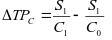
\includegraphics[width=0.7\textwidth]{assets/342}
	\caption*{Рисунок 1 - Воздействие вредных факторов на работников}
	\caption*{\normalfont \emph{Примечание -- составлено авторами}}
\end{figure}

Высокий удельный вес работающих во вредных условиях труда в этих
секторах обоснованы следующими факторами: усложненными технологическими
процессами, использованием тяжелого оборудования и взрывчатых веществ,
экстремальными температурами, воздействием токсичных веществ и др.
(рисунок 2)

\begin{figure}[H]
	\centering
	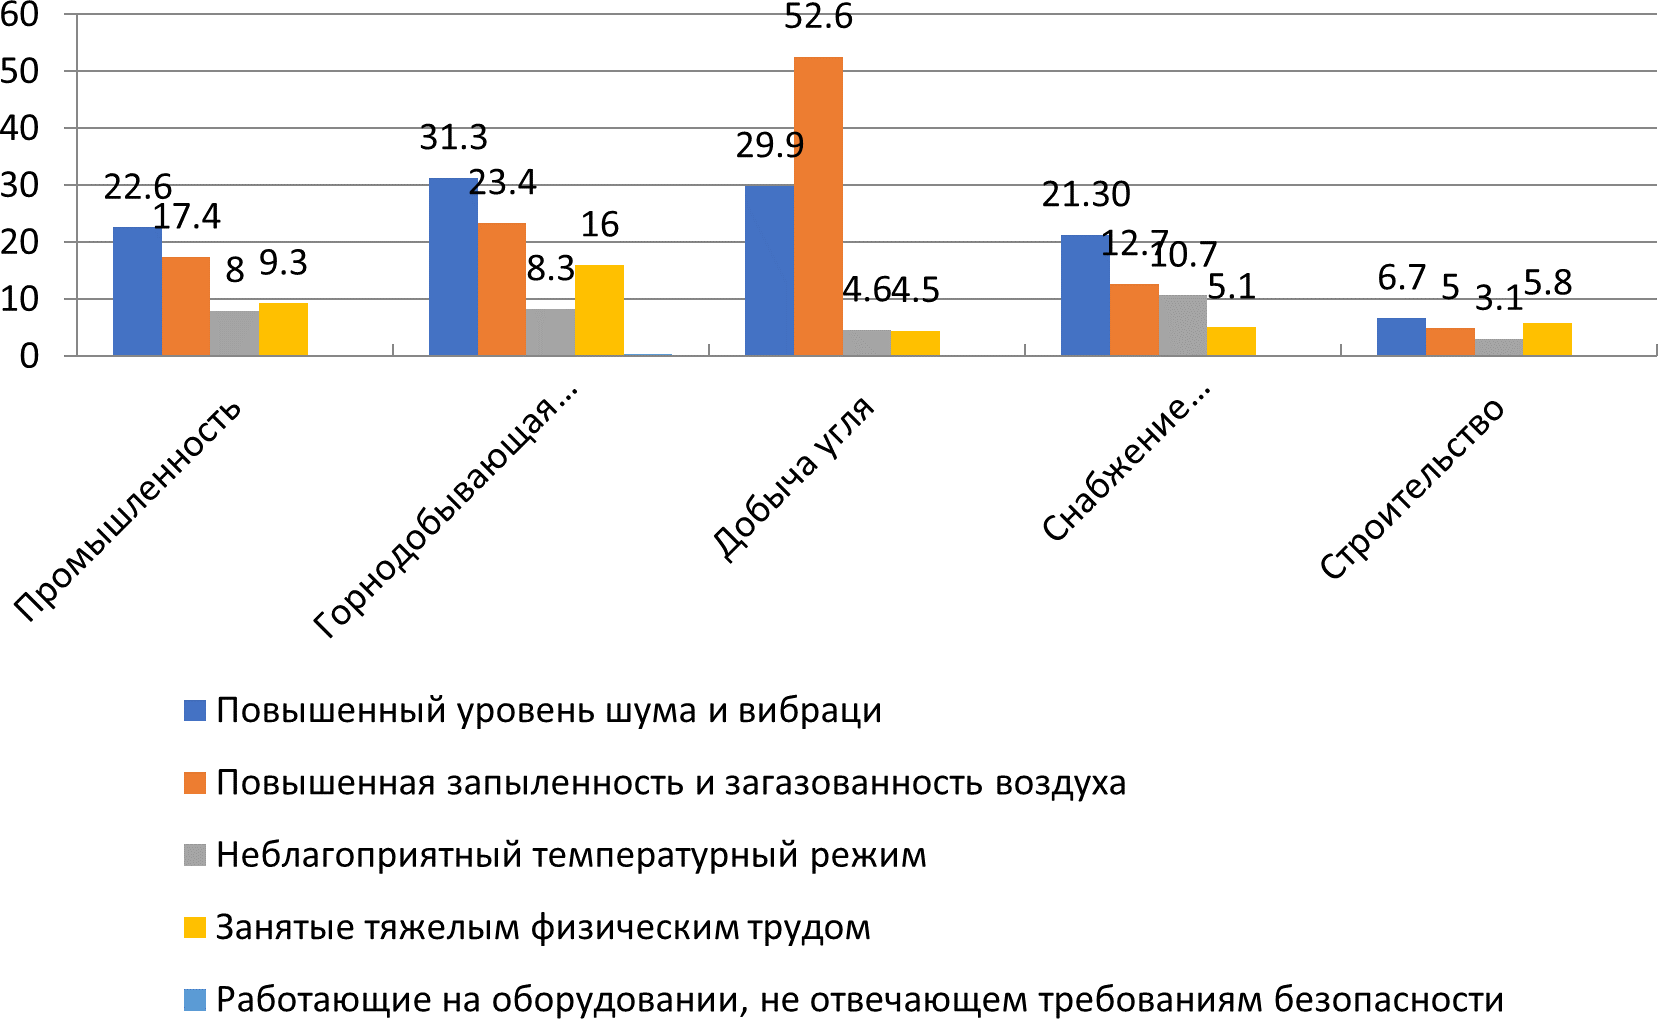
\includegraphics[width=0.7\textwidth]{assets/342.1}
	\caption*{Рис.2 - Удельный вес работников, занятых во вредных и других
неблагоприятных условиях труда}
	\caption*{\normalfont \emph{Примечание -- составлено авторами на основании статистических данных {[}16{]}}}
\end{figure}

\begin{multicols}{2}
Физическое воздействие

Заболевания и травмы. Вредные факторы, такие как шум, вибрация,
запыленность и загазованность воздуха, экстремальные температуры, могут
вызвать острые и хронические заболевания.

Снижение работоспособности. Воздействие вредных факторов может привести
к быстрой утомляемости, снижению физической выносливости и общей
работоспособности. Это, в свою очередь, повышает риск производственных
травм и аварий.

Психологическое воздействие

Стресс и утомляемость. Вредные факторы, такие как шум и вибрация, могут
вызывать повышенный стресс и утомляемость, что негативно сказывается на
психическом здоровье работников. Хронический стресс может привести к
развитию депрессии, тревожных расстройств и других психических
заболеваний.

Снижение концентрации и когнитивных функций. Шум и вибрация могут
снижать концентрацию внимания и когнитивные функции, что затрудняет
выполнение сложных и требующих внимания задач.

Социальное и экономическое воздействие

Снижение качества жизни. Хронические заболевания и психическое
напряжение, вызванные вредными факторами труда, могут снижать общее
качество жизни работников, ограничивая их физические и социальные
возможности.

Экономические потери. Заболевания и травмы работников приводят к потерям
рабочего времени, увеличению расходов на медицинское обслуживание и
снижению производительности труда. Это оказывает негативное влияние на
экономические показатели предприятий и национальной экономики в целом.

Анализ данных по вредным условиям труда показывает, что наибольший
удельный вес в добыче угля составляет запыленность и загазованность
воздуха, достигая 52,6\%. Этот фактор является наиболее значимым и
негативно влияет на дыхательную систему работников, увеличивая риск
развития хронических заболеваний легких. В горнодобывающей
промышленности и разработке карьеров наиболее выражены факторы шума и
вибрации, с показателем 31,3\%, и запыленности воздуха - 23,4\%. Эти
условия связаны с использованием тяжелого оборудования и взрывчатых
веществ, что повышает риск профессиональных заболеваний и травм.

Факторы шума и вибрации, запыленности и загазованности воздуха, а также
неблагоприятные температурные условия являются наиболее значимыми
вредными факторами в данных секторах экономики. Эти условия требуют
особого внимания к улучшению условий труда и внедрению мер по охране
здоровья работников.

Социальные гарантии в Республике Казахстан представляют дополнительный
отпуск, сокращенный рабочий день, повышенный размер оплаты труда,
обязательные профессиональные взносы и пр.) предоставляются на основе
списочного подхода с подтверждением результатами аттестации
производственных объектов по условиям труда

Необходимо отметить, что в 2023 году из 1 692 214 человек, работающих во
вредных условиях труда, 680 160 работников, было установлена хотя бы
одна из компенсаций. На сегодняшний день в Казахстане существуют
следующие виды компенсаций:

\begin{itemize}
\item
  дополнительные отпуска;
\item
  сокращенный рабочий день;
\item
  лечебно-профилактическое питание;
\item
  молоко и равноценные пищевые продукты;
\item
  доплаты за вредные и другие неблагоприятные условия труда.
\end{itemize}

Общая сумма затрат на компенсации за работу во вредных и других
неблагоприятных условиях труда по всем видам экономической деятельности
составляет 207 631 773 тыс. тенге. Структура компенсаций за работу во
вредных и других неблагоприятных условиях труда представлена на рисунке
3.
\end{multicols}

\begin{figure}[H]
	\centering
	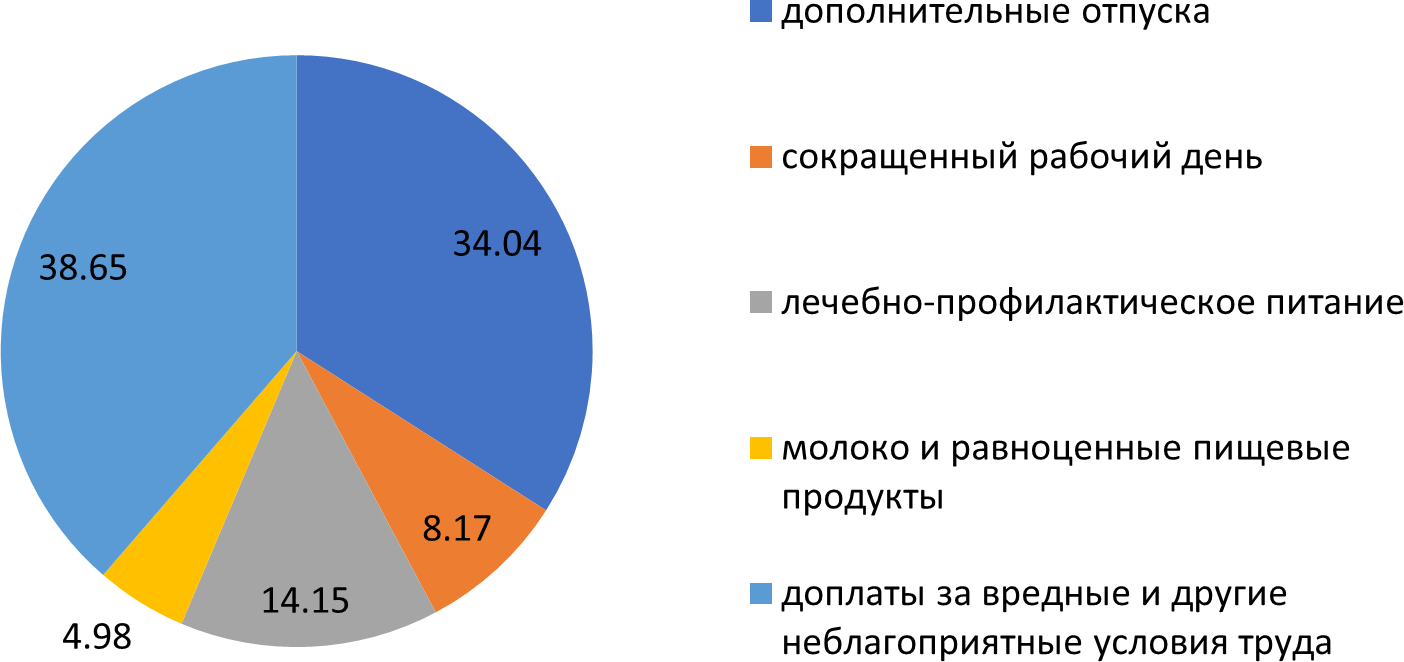
\includegraphics[width=0.7\textwidth]{assets/342.2}
	\caption*{Рис. 3 -- Структура компенсаций за работу во вредных и других неблагоприятных условиях труда}
	\caption*{\normalfont \emph{Примечание -- составлено авторами на основании статистических данных {[}16{]}}}
\end{figure}

\begin{multicols}{2}
Доплаты за вредные условия труда и дополнительные отпуска составляют
наибольшую долю в части компенсаций (38,65\% и 34,04\% соответственно).
Это свидетельствует о том, что развиваются циклические и дополнительные
отпуска, которые являются возможными мерами поддержки производителей.
Лечебно-профилактическое питание составляет 14,15\% от общей структуры
компенсаций, что обеспечивает измерение меры по сохранению здоровья
через специальное питание. Меньшая доля приходится на сокращенный
рабочий день и предоставление молока. Сокращенный рабочий день и
прибавка молока составляют меньшую долю в общей шкале компенсаций
(соответственно 8,17\% и 4,98\%). Это может быть связано с тем, что
применяются некоторые ограничения или особенности.

Для выявления диспропорций и несправедливостей был проведен
сравнительный анализ, позволяющий выявить возможные несоответсвия в
предоставлении компенсаций между мужчинами и женщинами, а также между
работниками различных форм собственности. Это важно для разработки
рекомендаций по устранению таких несправедливостей и обеспечения равных
условий труда для всех работников.

В государственной собственности общее количество работников, которым
установлены компенсации за работу во вредных условиях, составляет 196
935 человек, что составляет 28.95\% от общего числа работников, занятых
во вредных условиях труда в данном секторе. Из них 66 993 мужчины
(14.51\%) и 129 942 женщины (59.51\%).
\end{multicols}

\begin{longtable}[c]{|llllllll|}
\caption*{Таблица 2 -- Анализ данных по численности работников и компенсациям в Республике Казахстан} \\
\hline
\multicolumn{1}{|l|}{\multirow{2}{*}{}} &
  \multicolumn{2}{p{0.16\textwidth}|}{государственная собственность} &
  \multicolumn{2}{p{0.2\textwidth}|}{частная собственность} &
  \multicolumn{2}{p{0.16\textwidth}|}{иностранная собственность} &
  \multicolumn{1}{|p{0.1\textwidth}|}{всего} \\ \cline{2-8} 
\multicolumn{1}{|l|}{} &
  \multicolumn{1}{l|}{чел.} &
  \multicolumn{1}{l|}{\%} &
  \multicolumn{1}{l|}{чел.} &
  \multicolumn{1}{l|}{\%} &
  \multicolumn{1}{l|}{чел.} &
  \multicolumn{1}{l|}{\%} &
   \\ \hline
\endfirsthead
%
\endhead
%
\multicolumn{1}{|p{0.2\textwidth}|}{Численность работников, занятых во вредных и других неблагоприятных условиях труда по регионам} &
  \multicolumn{1}{l|}{457 874} &
  \multicolumn{1}{l|}{27,399} &
  \multicolumn{1}{l|}{1017417} &
  \multicolumn{1}{l|}{60,881} &
  \multicolumn{1}{l|}{195858} &
  \multicolumn{1}{l|}{11,72} &
  1 671 149 \\ \hline
\multicolumn{1}{|l|}{мужчины} &
  \multicolumn{1}{l|}{150 887} &
  \multicolumn{1}{l|}{15,122} &
  \multicolumn{1}{l|}{701667} &
  \multicolumn{1}{l|}{70,322} &
  \multicolumn{1}{l|}{145235} &
  \multicolumn{1}{l|}{14,556} &
  997 789 \\ \hline
\multicolumn{1}{|l|}{женщины} &
  \multicolumn{1}{l|}{306 987} &
  \multicolumn{1}{l|}{45,59} &
  \multicolumn{1}{l|}{315750} &
  \multicolumn{1}{l|}{46,892} &
  \multicolumn{1}{l|}{50623} &
  \multicolumn{1}{l|}{7,518} &
  673 360 \\ \hline
\multicolumn{1}{|p{0.2\textwidth}|}{Численность работников, которым за работу во вредных и других неблагоприятных условиях труда установлены компенсации} &
  \multicolumn{1}{l|}{196935} &
  \multicolumn{1}{l|}{28,954} &
  \multicolumn{1}{l|}{383716} &
  \multicolumn{1}{l|}{56,416} &
  \multicolumn{1}{l|}{99509} &
  \multicolumn{1}{l|}{14,63} &
  680 160 \\ \hline
\multicolumn{1}{|l|}{мужчины} &
  \multicolumn{1}{l|}{66993} &
  \multicolumn{1}{l|}{14,507} &
  \multicolumn{1}{l|}{311888} &
  \multicolumn{1}{l|}{67,536} &
  \multicolumn{1}{l|}{82928} &
  \multicolumn{1}{l|}{17,957} &
  461 809 \\ \hline
\multicolumn{1}{|l|}{женщины} &
  \multicolumn{1}{l|}{129942} &
  \multicolumn{1}{l|}{59,511} &
  \multicolumn{1}{l|}{71828} &
  \multicolumn{1}{l|}{32,896} &
  \multicolumn{1}{l|}{16581} &
  \multicolumn{1}{l|}{7,5937} &
  218 351 \\ \hline
\multicolumn{1}{|p{0.2\textwidth}|}{Сумма затрат на компенсации за работу во вредных и других неблагоприятных условиях труда по отдельным видам экономической деятельности (тыс.тенге)} &
  \multicolumn{1}{l|}{39314722} &
  \multicolumn{1}{l|}{18,935} &
  \multicolumn{1}{p{0.08\textwidth}|}{128 998 360,7} &
  \multicolumn{1}{l|}{62,128} &
  \multicolumn{1}{p{0.08\textwidth}|}{39 318 690} &
  \multicolumn{1}{l|}{18,937} &
  \multicolumn{1}{p{0.08\textwidth}|}{207 631 773} \\ \hline
\multicolumn{8}{|l|}{Примечание – составлено авторами на основании статистических данных {[}16{]}} \\ \hline
\end{longtable}

\begin{multicols}{2}
В частной собственности общее количество работников, которым установлены
компенсации, составляет 383 716 человек, что составляет 56.42\% от
общего числа работников, занятых во вредных условиях труда в частном
секторе. Из них 311 888 мужчины (67.54\%) и 71 828 женщины (32.90\%).

В иностранной собственности общее количество работников, которым
установлены компенсации, составляет 99 509 человек, что составляет
14.63\% от общего числа работников, занятых во вредных условиях труда в
иностранных компаниях. Из них 82 928 мужчины (17.96\%) и 16 581 женщины
(7.59\%) (таблица 2).

Государственные предприятия в 2023 году предоставили компенсации 28,95\%
работников, занятых во вредных условиях труда. Женщины в государственном
секторе получили компенсации чаще, чем мужчины, что может
свидетельствовать о большей концентрации женщин в работах, подлежащих
компенсации. Частные организации обеспечили компенсациями 56,42\%
работников, занятых во вредных условиях труда. В частном секторе в 2023
году значительно больше мужчин получили компенсации, чем женщины, что
может указывать на преобладание мужчин в профессиях с вредными условиями
труда, либо на более высокие компенсационные ставки для мужчин. В
иностранных компаниях компенсации были установлены для 14,63\%
работников. Подобно частному сектору, в иностранных компаниях
компенсации больше получили мужчины, что также может быть связано с
типами работ и условиями труда в этих предприятиях.

В государственной собственности часто наблюдается меньший уровень
компенсаций по сравнению с частными и иностранными предприятиями. Это
может быть связано с более строгими бюджетными ограничениями, сложными
бюрократическими процедурами и недостаточной информированностью
работников о своих правах. В частных и иностранных компаниях, напротив,
компенсации предоставляются чаще и в большем объеме, что может
объясняться лучшими финансовыми возможностями и желанием этих
предприятий привлекать и удерживать квалифицированных сотрудников.

Несоответствие в выплатах компенсаций отображается на всей системе
социальных гарантий, что указывает на существующие проблемы механизме
предоставления социальных гарантий. Это требует пересмотра и улучшения
существующих механизмов предоставления компенсаций и социальных
гарантий, чтобы обеспечить равные и справедливые условия для всех
работников, независимо от формы собственности предприятия. Улучшение
системы социальных гарантий будет способствовать созданию более
безопасных и здоровых условий труда, что положительно скажется на общем
состоянии производственной среды и благосостоянии работников.

На сегодняшний момент, социальные гарантии в Казахстане предоставляются
на основе списочного подхода с подтверждением результатами аттестации
производственных объектов по условиям труда. Социальные гарантии для
работников, занятых на тяжелых и вредных производствах, предоставляются
на основе списочного подхода и подтверждаются результатами аттестации
производственных объектов по условиям труда.

Однако можно отметить, что процедура проведения аттестации
производственных объектов по условиям труда проводится не всегда
качественно и не отражает фактические условия труда, также не учитывает
риски и дифференциацию для каждого рабочего места.

Кроме того, отсутствие единого подхода к оценке условий труда и
критериев для проведения аттестации приводит к неоднородности в
применении социальных гарантий. Это, в свою очередь, создает предпосылки
для несправедливого распределения компенсаций и льгот, что может
вызывать социальную напряженность среди работников.

Для решения этих проблем необходимо пересмотреть текущую систему
аттестации рабочих мест с целью обеспечения её объективности и
прозрачности. Это может включать в себя следующие шаги:

\begin{itemize}
\item
  Разработка единых стандартов и критериев оценки условий труда.
  Введение унифицированных правил и процедур, которые будут применяться
  ко всем предприятиям независимо от их формы собственности, позволит
  создать более справедливую систему оценки.
\item
  Усиление контроля за проведением аттестации. Создание независимых
  органов или комиссий, которые будут проводить регулярные проверки
  качества аттестации производственных объектов, поможет минимизировать
  ошибки и злоупотребления.
\item
  Внедрение дифференцированного подхода к оценке рабочих мест. Учет
  специфики каждого рабочего места и индивидуальных рисков позволит
  более точно определить необходимый уровень компенсаций и социальных
  гарантий.
\item
  Обучение и повышение квалификации специалистов по охране труда.
  Повышение уровня подготовки кадров, занимающихся аттестацией,
  гарантирует, что результаты будут более достоверными и
  соответствующими реальным условиям труда.
\item
  Разработка системы обратной связи для работников. Введение механизмов,
  позволяющих работникам сообщать о несоответствиях в условиях труда и в
  оценке их рабочих мест, поможет оперативно выявлять и устранять
  проблемы.
\end{itemize}

Эти меры могут значительно повысить эффективность системы социальных
гарантий в Казахстане, сделав её более прозрачной, справедливой и
соответствующей реальным потребностям работников. В конечном итоге, это
приведет к улучшению условий труда, снижению уровня профессиональных
заболеваний и травматизма, а также к повышению общей удовлетворенности
трудящихся.

{\bfseries Выводы.} Проведенное исследование подтвердило наличие
значительных проблем в системе предоставления социальных гарантий для
работников, занятых на вредных и опасных производствах в Республике
Казахстан. Основные выводы можно сформулировать следующим образом:

\begin{itemize}
\item
  неоднородность предоставления социальных гарантий. Исследование
  показало, что существующая система оценки условий труда и последующая
  аттестация производственных объектов часто не отражают реальные
  условия труда. Это приводит к неравномерному распределению компенсаций
  и льгот среди работников различных форм собственности и секторов
  экономики.
\item
  недостатки в системе аттестации рабочих мест. Отсутствие единых
  стандартов и критериев для оценки условий труда ведет к возникновению
  значительных различий в результатах аттестации, что создает
  предпосылки для несправедливого распределения социальных гарантий.
\item
  необходимость пересмотра и совершенствования механизмов. Для
  обеспечения равных и справедливых условий труда необходимо
  пересмотреть текущие механизмы предоставления социальных гарантий.
  Внедрение дифференцированного подхода к оценке рабочих мест и усиление
  контроля за проведением аттестации может существенно улучшить
  ситуацию.
\item
  рекомендации по улучшению системы социальных гарантий. Важным шагом в
  этом направлении является разработка унифицированных правил и
  процедур, которые будут применяться ко всем предприятиям, а также
  создание независимых органов для контроля за качеством аттестации.
  Дополнительно, обучение и повышение квалификации специалистов по
  охране труда могут значительно повысить достоверность оценки условий
  труда.
\end{itemize}

\emph{{\bfseries Финансирование.} В статье изложены результаты
исследований, полученных в ходе реализации научно-технической программы
на тему «Трансформация государственного механизма социальных гарантий в
отношении лиц, занятых во вредных условиях труда в современном
контексте» (ИРН AP23490760).}
\end{multicols}

\begin{center}
{\bfseries Литература}
\end{center}

\begin{noparindent}
1.Трудовой кодекс Республики Казахстан -
https://adilet.zan.kz/rus/docs/K1500000414

2.Об утверждении перечня производств, работ, профессий работников,
занятых на работах с вредными условиями труда, в пользу которых агентами
по уплате обязательных профессиональных пенсионных взносов за счет
собственных средств осуществляются обязательные профессиональные
пенсионные взносы - https://adilet.zan.kz/rus/docs/V2300032568

3.Закон Республики Казахстан О внесении изменений и дополнений в
некоторые законодательные акты Республики Казахстан по вопросам
общественных объединений и социальной защиты лиц, занятых на работах с
вредными условиями труда -
https://online.zakon.kz/Document/?doc\_id=35874764

4.А. М. Елин, С. С. Сергеева Специальная оценка условий труда: практика
и итоги//Нормативные акты и документы - № 2 (92) 2020, март-апрель -- с.
52-59 DOI 10.18635/2071-2219-2020-2-52-59

5.Хайруллина Л.И., Гасилов В.С. Компенсации за работу во вредных
условиях труда: основные аспекты вопроса // Фундаментальные
исследования. 2019. URL:

https://s.fundamental-research.ru/pdf/2019/7/42523.pdf (дата обращения:
22.08.2024).

6.Ильин С.М., Самарская Н.А., Симанович С.В., Сергеева С.С. Направления
совершенствования системы предоставления гарантий и компенсаций
работникам за работу в опасных (вредных) условиях труда // Экономика
труда. -- 2021. -- Том 8. -- № 9. -- С. 1055--1074. doi:
10.18334/et.8.9.113564

7.Божков А.Д. Аналитическая оценка эффективности затрат на улучшение
мероприятий по охране труда на ООО «Меганом» Аллея науки. 2018. Т. 1. №
5 (21). С. 462-466.

8.Рыбалченко К.Ю., Бухтояров В.Ф. Зависимости между затратами на охрану
труда и показателями производственного электротравматизма (на примере
южно-уральской железной дороги) // Фундаментальные исследования. 2013. №
8-1. С. 49-52.

9.Дождева А.А. Мировой опыт формирования затрат на охрану и условия
трудам - В сборнике: Современные проблемы экономического развития.
Материалы Всероссийской научной студенческой конференции. Отв. ред. Е.А.
Кипервар. 2019. С. 89-95.

10.Абикенова Ш.К., Айткенова Г.Т., Махатов Е.М., Кенжебаева К.М.
Разработка классификации затрат на охрану труда - В сборнике:
Приоритетные направления развития науки и образования. сборник статей XX
Международной научно-практической конференции. Пенза, 2021. С. 96-98.

11.Еселханова Г.А., Танабаева А.Е. Нормативно-правовое регулирование
предоставления гарантий работникам, занятым во вредных и опасных
условиях труда в Республике Казахстан// Научное обозрение • Технические
науки № 1, 2017 -- с. 71-74

12.С.М. Базарбаева, С.Т. Шорманов, С.Т. Толеугали «Анализ действующего
механизма регулирования труда лиц, занятых в неблагоприятных условиях»//

Наука и мир. 2017. № 11 (51). Vol. I. -- с.26-27

13.Muhammad Ajmal, Ahmad Shahrul Nizam Isha, Shahrina Md Nordin «Safety
Management Practices and Occupational Health and Safety Performance: An
Empirical Review»// Jinnah Business Review - July 2021, Vol. 9, No. 2,
pp. 15-33 DOI:10.53369/DTOC3606

14.Effect of Occupational Health and Safety Management System on
Work-Related Accident Rate and Differences of Occupational Health and
Safety Management System Awareness between Managers in South
Korea\textquotesingle s Construction Industry.

15.Liu, S., Nkrumah, E. N. K., Akoto, L. S., Gyabeng, ., and Nkrumah, E.
(2020). The state of occupational health and safety management
frameworks (ohsmf) and occupational injuries and accidents in the
ghanaian oil and gas industry: assessing the mediating role of safety
knowledge. BioMed research international, 2020.

16.https://stat.gov.kz/ru/industries/labor-and-income/stat-wags/
\end{noparindent}

\begin{center}
{\bfseries References}
\end{center}

\begin{noparindent}
1.Trudovoj kodeks Respubliki Kazahstan -
https://adilet.zan.kz/rus/docs/K1500000414

2.Ob utverzhdenii perechnja proizvodstv, rabot, professij rabotnikov,
zanjatyh na rabotah s vrednymi uslovijami truda, v
pol\textquotesingle zu kotoryh agentami po uplate
objazatel\textquotesingle nyh professional\textquotesingle nyh
pensionnyh vznosov za schet sobstvennyh sredstv osushhestvljajutsja
objazatel\textquotesingle nye professional\textquotesingle nye
pensionnye vznosy -

https://adilet.zan.kz/rus/docs/V2300032568

3.Zakon Respubliki Kazahstan O vnesenii izmenenij i dopolnenij v
nekotorye zakonodatel\textquotesingle nye akty Respubliki Kazahstan po
voprosam obshhestvennyh ob\#edinenij i social\textquotesingle noj
zashhity lic, zanjatyh na rabotah s vrednymi uslovijami truda -
https://online.zakon.kz/Document/?doc\_id=35874764

4.A. M. Elin, S. S. Sergeeva Special\textquotesingle naja ocenka uslovij
truda: praktika i itogi//Normativnye akty i dokumenty - № 2 (92) 2020,
mart-aprel\textquotesingle{} -- s. 52-59 DOI
10.18635/2071-2219-2020-2-52-59

5.Hajrullina L.I., Gasilov V.S. Kompensacii za rabotu vo vrednyh
uslovijah truda: osnovnye aspekty voprosa //
Fundamental\textquotesingle nye issledovanija. 2019. URL:
https://s.fundamental-research.ru/pdf/2019/7/42523.pdf (data
obrashhenija: 22.08.2024).

6.Il\textquotesingle in S.M., Samarskaja N.A., Simanovich S.V., Sergeeva
S.S. Napravlenija sovershenstvovanija sistemy predostavlenija garantij i
kompensacij rabotnikam za rabotu v opasnyh (vrednyh) uslovijah truda //
Jekonomika truda. -- 2021. -- Tom 8. -- № 9. -- S. 1055--1074. doi:
10.18334/et.8.9.113564

7.Bozhkov A.D. Analiticheskaja ocenka jeffektivnosti zatrat na
uluchshenie meroprijatij po ohrane truda na OOO «Meganom» Alleja nauki.
2018. T. 1. № 5 (21). S. 462-466.

8.Rybalchenko K.Ju., Buhtojarov V.F. Zavisimosti mezhdu zatratami na
ohranu truda i pokazateljami proizvodstvennogo jelektrotravmatizma (na
primere juzhno-ural\textquotesingle skoj zheleznoj dorogi) //
Fundamental\textquotesingle nye issledovanija. 2013. № 8-1. S. 49-52.

9.Dozhdeva A.A. Mirovoj opyt formirovanija zatrat na ohranu i uslovija
trudam - V sbornike: Sovremennye problemy jekonomicheskogo razvitija.
Materialy Vserossijskoj nauchnoj studencheskoj konferencii. Otv. red.
E.A. Kipervar. 2019. S. 89-95.

10.Abikenova Sh.K., Ajtkenova G.T., Mahatov E.M., Kenzhebaeva K.M.
Razrabotka klassifikacii zatrat na ohranu truda - V sbornike:
Prioritetnye napravlenija razvitija nauki i obrazovanija. sbornik statej
XX Mezhdunarodnoj nauchno-prakticheskoj konferencii. Penza, 2021. S.
96-98.

11.Eselhanova G.A., Tanabaeva A.E. Normativno-pravovoe regulirovanie
predostavlenija garantij rabotnikam, zanjatym vo vrednyh i opasnyh
uslovijah truda v Respublike Kazahstan// Nauchnoe obozrenie •
Tehnicheskie nauki № 1, 2017 -- s. 71-74

12.S.M. Bazarbaeva, S.T. Shormanov, S.T. Toleugali «Analiz
dejstvujushhego mehanizma regulirovanija truda lic, zanjatyh v
neblagoprijatnyh uslovijah»//

13.Muhammad Ajmal, Ahmad Shahrul Nizam Isha, Shahrina Md Nordin «Safety
Management Practices and Occupational Health and Safety Performance: An
Empirical Review»// Jinnah Business Review - July 2021, Vol. 9, No. 2,
pp. 15-33 DOI:10.53369/DTOC3606

14.Effect of Occupational Health and Safety Management System on
Work-Related Accident Rate and Differences of Occupational Health and
Safety Management System Awareness between Managers in South
Korea\textquotesingle s Construction Industry.

15.Liu, S., Nkrumah, E. N. K., Akoto, L. S., Gyabeng, ., and Nkrumah, E.
(2020). The state of occupational health and safety management
frameworks (ohsmf) and occupational injuries and accidents in the
ghanaian oil and gas industry: assessing the mediating role of safety
knowledge. BioMed research international, 2020.

16.https://stat.gov.kz/ru/industries/labor-and-income/stat-wags/
\end{noparindent}

\emph{{\bfseries Сведения об авторах}}

\begin{noparindent}
Курманов А.М.- к.э.н., генеральный директор Республиканского
научно-исследовательский институт по охране труда Министерства труда и
социальной защиты населения Республики Казахстан, Астана, e-mail:
rniiot@rniiot.kz;

Сарыбаева И.Е.-докторант Евразийского национального университета имени
Л.Н. Гумилева, Астана, Казахстан, e-mail: inarasaribaeva@gmail.com;

Омаркожаева А.Н.- к.э.н., доцент Казахский университет технологии и
бизнеса им.К.Кулажанова, Астана, Казахстан, e-mail: asya\_7510@mail.ru;

Бекмагамбетов А.Б. -- к.ю.н., ассоциированный профессор, зам.
генерального директора Республиканского научно-исследовательский
институт по охране труда Министерства труда и социальной защиты
населения Республики, e-mail: adilet1979@mail.ru
\end{noparindent}

\emph{{\bfseries Information about the authors}}

\begin{noparindent}
A.M.Kurmanov - Candidate of Economic Sciences, CEO, General Director of
the Republican Research Institute for Labor Protection of the Ministry
of Labor and Social Protection of the Population of the Republic
Kazakhstan, e-mail: rniiot@rniiot.kz;

I.E. Sarybayeva -- PhD student of L.N. Gumilyov Eurasian National
University, Astana, e-mail:

inarasaribaeva@gmail.com;

A.N. Omarkozhayeva - Candidate of Economic Sciences, Associate
Professor, K.Kulazhanov Kazakh University of Technology and Business,
Astana, Kazakhstan, e-mail: asya\_7510@mail.ru;

A.B.Bekmagambetov - Candidate of Legal Sciences, Associate Professor,
Deputy Director General of the Republican Scientific Research Institute
for Labor Protection of the Ministry of Labor and Social Protection of
the Population of the Republic Kazakhstan, e-mail: adilet1979@mail.ru
\end{noparindent}
